% !TEX root = ../thesis.tex

\chapter{Methodology}
\label{chap:model}
We choose deep learning for our task. In contrast to conventional vision learning methods, deep learning methods not only learn a classification model but also a holistic representation of the raw image or video input, which liberates the user from exhaustive pre- and post-processing, hence opens the door to a series of online applications for this field of study. 
Moreover, deep neural networks are able to extract high level semantic features, which is critical in dealing with abstract concepts like action. 

In order to separate semantic structures, we adopt the method in R*CNN \cite{gkioxari2015contextual}, which utilizes the concept of regional pooling initially proposed by \cite{girshick2015fast}.

While ground truth person bounding boxes is available in R*CNN, we only have action labels for each video sequence. We employ state-of-art object detector Faster-RCNN \cite{ren2015faster} for person and object detection.

To handle detection failure due to motion blur, extreme pose variation or occlusion and additionally filter out persons irrelevant to the action, we use Dynamic Programming on frame-wise detections to estimate a smooth person trajectory through the video sequence.

Finally we train our network using settings and techniques suggested in \cite{wang2015towards} and delve into various fusion methods to maximize the complementary effect of different cues.

The rest of this chapter is organized as follows: 
\begin{itemize}
\item in \autoref{sec:modelarch} we give a comprehensive insight into our model architecture;
\item in \autoref{sec:detection} we provide an overview on Faster-RCNN as well as a recap over our post-processing on raw detection results.
\item finally in \autoref{sec:fusion} we propose various fusion methods and describe the motivations behind each of them.
\end{itemize}
 

\section{Model Architecture}\label{sec:modelarch}
\begin{figure}
\centering
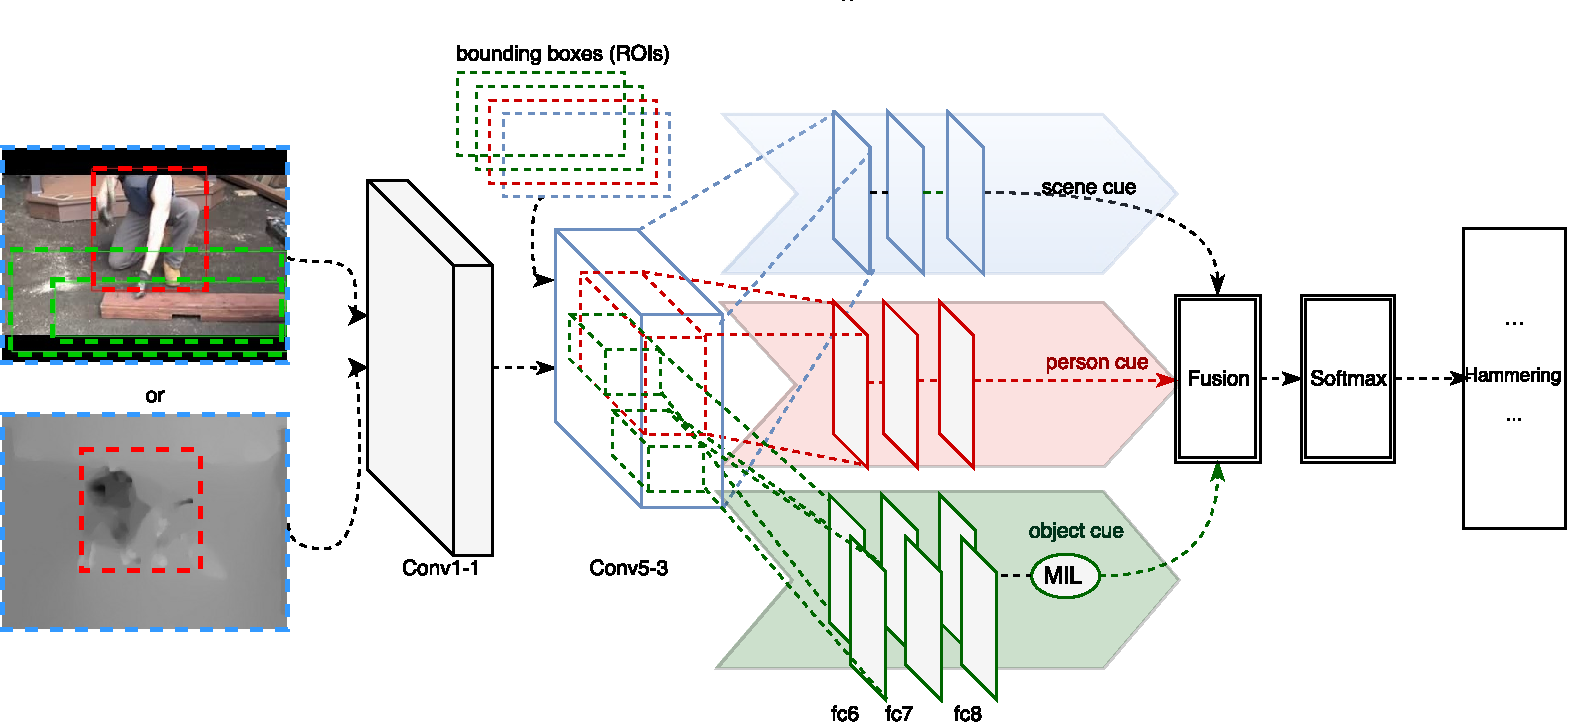
\includegraphics[width=\linewidth]{figures/net.pdf}
\caption[Network Architecture]{The general architecture of our network. Semantic cues (scene, person and objects) are integrated as pooling regions to create explicit semantic structures (parallel fc layers). The classification results from each semantic channel are merged in a fusion unit as well be discussed in \autoref{sec:fusion}.}
\label{fig:net}
\end{figure}
The general setting of our network architecture is illustrated in \autoref{fig:net}. It is composed of three parts.

The first part of our model is comprised of very deep convolutional layers. 
We adopt VGG16 configuration proposed by \cite{simonyan2014very}. 
This publicly available network is trained on ImageNet data for the ILSVRC2012 \cite{ILSVRC15} challenge and has been used as initialization network for various tasks.
A total of 13 convolutional layers and 3 fully connected layers are implemented. For clarity, its specifications are recapped in \autoref{tab:vgg16}.
\begin{table}
\centering\small
\begin{tabular}{m{0.2\linewidth}|m{0.3\linewidth}|m{0.2\linewidth}}
\hline
Layer & Param & Effective \newline Receptive Field \\ \hline
Conv1-1 \newline Conv1-2 & $ \begin{aligned}
k &= 2\times 2, & n &= 64,\\
p &= 1, & s &= 1 \end{aligned} $ & 3\\ \hline
MaxPool & $ \begin{aligned}
k & = 2 \times 2, &s &= 2
\end{aligned}$ & 6\\ \hline
Conv2-1 \newline Conv2-2 & $ \begin{aligned}
k &= 3\times 3, & n &= 128,\\
p &= 1, & s &= 1 \end{aligned} $ &  14\\ \hline
MaxPool & $ \begin{aligned}
k & = 2 \times 2, &s &= 2
\end{aligned}$ & 20\\ \hline
Conv3-1 \newline Conv3-2 \newline Conv3-3 & 
$ \begin{aligned}
k &= 3\times 3, & n &= 256,\\
p &= 1, & s &= 1  \end{aligned} $ & 44\\ \hline
MaxPool & $ \begin{aligned}
k & = 2 \times 2, &s &= 2
\end{aligned}$ & 56\\ \hline
Conv4-1 \newline Conv4-2 \newline Conv4-3 & $ \begin{aligned}
k &= 3\times 3, & n &= 512,\\
p &= 1, & s &= 1  \end{aligned} $ & 104\\ \hline
MaxPool & $ \begin{aligned}
k & = 2 \times 2, &s &= 2
\end{aligned}$ & 128\\ \hline
Conv5-1 \newline Conv5-2 \newline Conv5-3 & $ \begin{aligned}
k &= 3\times 3, & n &= 512,\\
p &= 1, & s &= 1  \end{aligned} $ & 224\\ \hline
MaxPool  & $ \begin{aligned}
k & = 2 \times 2, &s &= 2
\end{aligned}$ & 272\\ \hline
fc6\newline Dropout  & $ \begin{aligned}
n & = 4096, & r &= 0.5
\end{aligned} $ & -\\ \hline
fc7\newline Dropout & $ \begin{aligned}
n & = 4096, & r &= 0.5
\end{aligned} $ & -\\ \hline
fc8  & $ \begin{aligned}
n & = 1000
\end{aligned} $ & -\\ \hline
\multicolumn{3}{c}{softmax} \\ \hline
\end{tabular}
\caption[VGG16 Configuration]{Configuration of Conv1 - Conv5 layers in VGG16. $ k $, $ n $, $ p $, $ s $ denote denote kernel size, number of output channels and padding and stride respectively. For the sake of brevity, ReLu layers, attached after every convolutional and fully connected layer, are omitted in the table.}
\label{tab:vgg16}
\end{table}
\subsection{Semantic decomposition using RoiPooling}
The second part of the network starts with a RoiPooling (Region Of Interest Pooling) layer (\cite{girshick2015fast}), which replaces the original MaxPooling after conv5-3.

Compared to regular pooling layers, which operate on the whole spatial span, the RoiPooling layer works in regions given at runtime. 
More concretely, it takes a series of rectangular regions as input and generates an independent feature map for each ROI by performing MaxPooling within the spatial area defined by each of these ROIs. 

Since the ROIs take on various sizes, a conventional pooling operation would output feature maps of different sizes. 
However the consecutive fully connected layer requires fixed input size.
In order to guarantee uniform output size, RoiPooling layer adopts adaptive bin size.
As is illustrated in \ref{fig:roipooling} (modified from \cite{kaiminghe}), given a ROI of size $ W \times H $ and the output feature map specified to be $ w \times h $ (in our case $ 7\times 7 $), RoiPooling first evenly divides the given ROIs into bins of size $ \lfloor\frac{W}{w}\rfloor \times \lfloor \frac{H}{h}\rfloor$ and then performs MaxPooling in each bin.

\begin{figure}
\centering
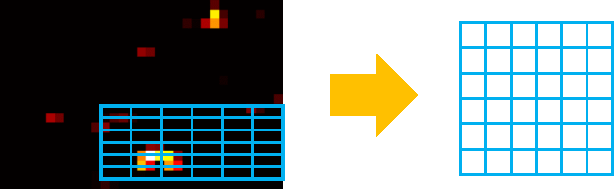
\includegraphics[width=0.7\linewidth]{figures/roipooling.pdf}
\caption[RoiPooling]{RoiPooling layer performs MaxPooling in regions of arbitrary size to a fixed size feature map by adapting the bin sizes.}\label{fig:roipooling}
\end{figure}

%\subcaptionbox{\label{fig:roipooling}}[0.6\linewidth]{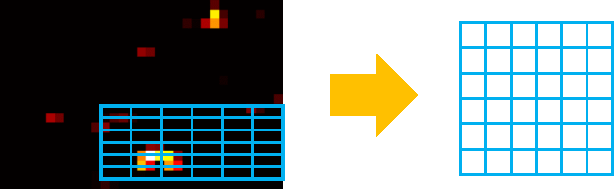
\includegraphics[width=0.6\linewidth]{figures/roipooling.pdf}}
%\subcaptionbox{\label{fig:irrelevantMIL}}[0.3\linewidth]{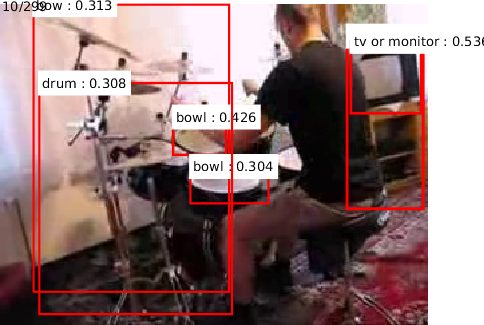
\includegraphics[width=0.3\linewidth]{figures/obj_detect1.png}}
%\begin{subfigure}[b]{0.6\linewidth}
%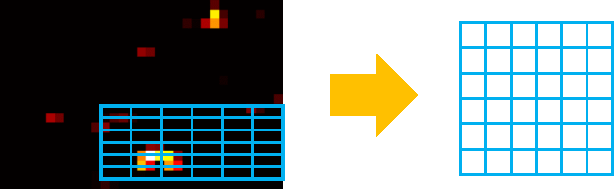
\includegraphics[width=0.9\columnwidth]{figures/roipooling.pdf}
%\caption[RoiPooling]{RoiPooling layer performs MaxPooling in regions of arbitrary size to a fixed size feature map by adapting the bin sizes.}\label{fig:roipooling}
%\end{subfigure}
%\begin{subfigure}[b]{0.3\linewidth}
%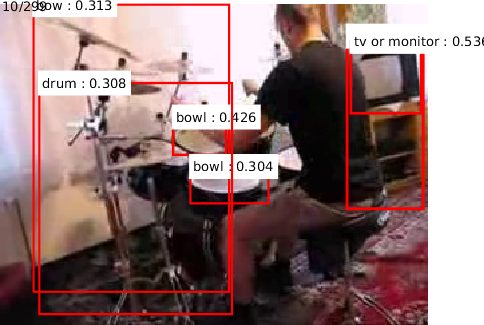
\includegraphics[width=0.9\columnwidth]{figures/obj_detect1.png}
%\caption[Example of object detections]{Example where the key object is mixed among many irrelevant objects.}\label{fig:irrelevantMIL}
%\end{subfigure}
%\caption[]{\subref{fig:roipooling} RoiPooling layer performs MaxPooling in regions of arbitrary size to a fixed size feature map by adapting the bin sizes. \subref{fig:irrelevantMIL} Example where the key object is mixed among many irrelevant objects.}\label{fig:roiandmil}
%\end{figure}

In accordance with our previous analysis, we group the ROIs into three categories, namely scene, person and objects. 
Depending on the category of ROIs, their feature maps are to be fed into one of the three fully connected branches representing each of the three cues respectively.
The underlying idea is simple: since the contribution of different semantic components are distinct, they should be handled separately. 
By leveraging the spatial  correspondence between feature maps and input images, we extract each cue on feature level, so as to train a more specialized classifier for each of them. 

As for the ROI inputs, we use an external object detector (see \autoref{sec:detection}) to generate person and object ROIs, while scene ROI is simply set to be the full input span $ \left(0, 0, W, H\right) $, in which case RoiPooling is equivalent to a regular MaxPooling.


For each input frame $ I $, exactly one person ROI and one scene ROI are used, while a variable number of ROIs are accepted for the object cue. 
This is due to the fact that in current datasets the defined action classes mostly involve only a single protagonist, while the contributing objects may be, and often are, multiple. 

\subsection{Object Channel with Multiple Instance Learning}
Often the decisive object, if detected at all, is mixed among many irrelevant detections (see \autoref{fig:irrelevantMIL}).
\begin{figure}
\centering
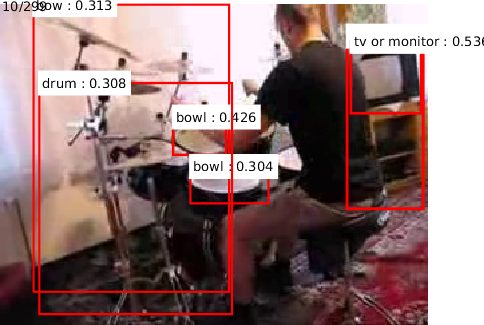
\includegraphics[width=0.5\linewidth]{figures/obj_detect1.png}
\caption[Example of object detections]{Example where the key object is mixed among many irrelevant objects.}\label{fig:irrelevantMIL}
\end{figure}
This described problem matches basic scenario in Multiple Instance Learning (MIL). 
In MIL, one is given bags of samples, called instances.
Unlike in conventional supervised learning problems, where each instance is labeled individually, labels are assigned to \textit{bags of} instances.
In the standard MIL assumption, a bag (and all its containing instances) is labeled positive, as long as there exists one positive instance in the bag; conversely, a bag is labeled negative, if all containing instances are negative.
The goal in MIL is to induce the underlying concept that will label individual instances correctly. 
In our case, bags translate to video frames, and instances are the detected objects.
Considering the previous example shown in \autoref{fig:irrelevantMIL}, all objects are labeled as "Drumming", although only "Drum" is the conclusive instance.

MIL has its own established field of study and it is not straightforward to transfer it directly to deep learning framework. 
While an abundance of algorithms has been developed, which implicitly or explicitly generalize the underlying MI assumption (\cite{foulds2010review}), they commonly leverage the most representative instance within a bag to encode the similarity of the bag to a candidate concept.
This similarity measurement is used to (a) find the desired concept alternately or (b) create a new feature space for bag representation, upon which a classifier can be trained to predict new bags.

In the scope of this thesis, we adopt the approach proposed by Gkioxari, which took inspiration from this aforementioned idea. 
In their work \cite{gkioxari2015contextual}, they combine multiple context regions, called secondary regions, using a MIL layer. For an input frame and a set of objects $ O $, the MIL layer computes the classification score for class $ c $ as:
\begin{equation}
s\left[c\right] = \max_{o\in O} s_{o}\left[c\right],
\end{equation}
where $  s_{o}\left[c\right] $ denotes the classification score of object $ o $ ROI for class $ c $. In other words, for each class the classification score of a frame (bag) is given by the object (instance) that is most representative for target class.
The back-propagation works similar to a normal MaxPooling layer. Derivatives from the upper layer will be passed down to (and only to) the instance from which the value was pooled, i.e.
\begin{equation}
\left[\derivative{L}{x_{i}}\right]_{c} = 
\lbrace i = \argmax_{n} x_{n}\left[c\right]\rbrace\left[\derivative{L}{y}\right]_{c},
\end{equation}
where $ \left[\derivative{L}{x_{i}}\right]_{c}  $ and $ \left[\derivative{L}{y}\right]_{c} $ denote the derivatives for class $ c $ and $ \lbrace i = \argmax_{n} x_{n}\left[c\right]\rbrace $ indicates whether the classification score for class $ c $ is pooled from this instance $ i $.
From the validation results reported in \cite{gkioxari2015contextual}, their model incorporating this MIL layer empirically improved the classification performance in PASCAL VOC action recognition challenge, although in-depth analysis over the influence of MIL is not provided.

\subsection{Fusion}
Finally, an independent classification score is produced by each branch of the fully connected layers. 
As the final part of our model, a merging unit combines them into a single classification score, which will be passed through a Softmax layer to obtain the actual class probabilities. 
Whereas R*CNN simply used sum merging, we implemented and empirically evaluated various of merging methods including sum, max, multiloss and weighted sum.
The detail of each variation will be given in \autoref{chap:setup}, while the results and analysis will be presented in \autoref{chap:result}.


\section{Human Object Detection}\label{sec:detection}
% !TEX root = ../thesis.tex
In this section, we describe our method for extracting reliable person and object bounding boxes.

\subsection{Object Detector Faster-RCNN}
The bounding boxes for objects and persons are extracted using the state-of-the-art object detector Faster-RCNN (Regional Convolutional Neural Network)\cite{ren2015faster}. 
Faster-RCNN is purely CNN-based state-of-the-art object detector that provides an end-to-end near real-time solution for object detection.

Faster-RCNN is an upgrade of Fast-RCNN. Compared to the latter, it significantly improves test-time speed by integrating regional object proposal into the system. As can be seen in the \autoref{fig:faster-rnn}, Faster-RCNN consists of two parts. The first part, \textit{Regional Proposal Net} (\textit{RPN}) takes an image as input and generates as output a set of rectangular regions with high objectness, called \textit{proposals}. 
The second part of the system, \textit{Detection Net} (DN), uses these proposals to compute the object location and predict the object class.

In both parts, object locations are parameterized as a 4-tuple  $ \mathbf{t} $, which specifies a scale-invariant translation and log-space height/width shift relative to a reference box $ a $ \cite{girshick2014rich}.
More specifically, the parameterization $ \mathbf{t} = \left(t_{x}, t_{y}, t_{w}, t_{h}\right) $ is defined as
\begin{equation}
\begin{aligned}\label{eq:bbtuple}
t_{x} &= (x-x_{a})/w_{a}\\
t_{y} &= (y-y_{a})/y_{a}\\
t_{w} &= \log(w/w_{a})\\
t_{h} &= \log(h/h_{a}),
\end{aligned}
\end{equation}
where $ x, y, w$ and $ h $ denote the center coordinates, width and height of a bounding box.

While both parts can be deployed as a standalone network for its own task, Faster-RCNN proposes a unified network that further improves test-time speed. 
More concretely, RPN and DN share the same convolutional layers. 
At test-time, an input image only needs to go through the convolutional layers once.
The output of the last shared convolutional layer is first used in RPN for proposal generation and then, together with RPN's output, in DN for detection.


The convolutional layers adopt the architecture in VGG16 (see \autoref{tab:vgg16}). The total stride at the last convolutional layer adds up to 16, i.e. an input image of the size $ W\times H $ will generate a $ \lceil \frac{W}{16}\rceil \times \lceil\frac{H}{16}\rceil \times K $ feature map, where $ K $ denotes the number of channels and equals $ 512 $ in VGG16.
\begin{figure}
	\centering
	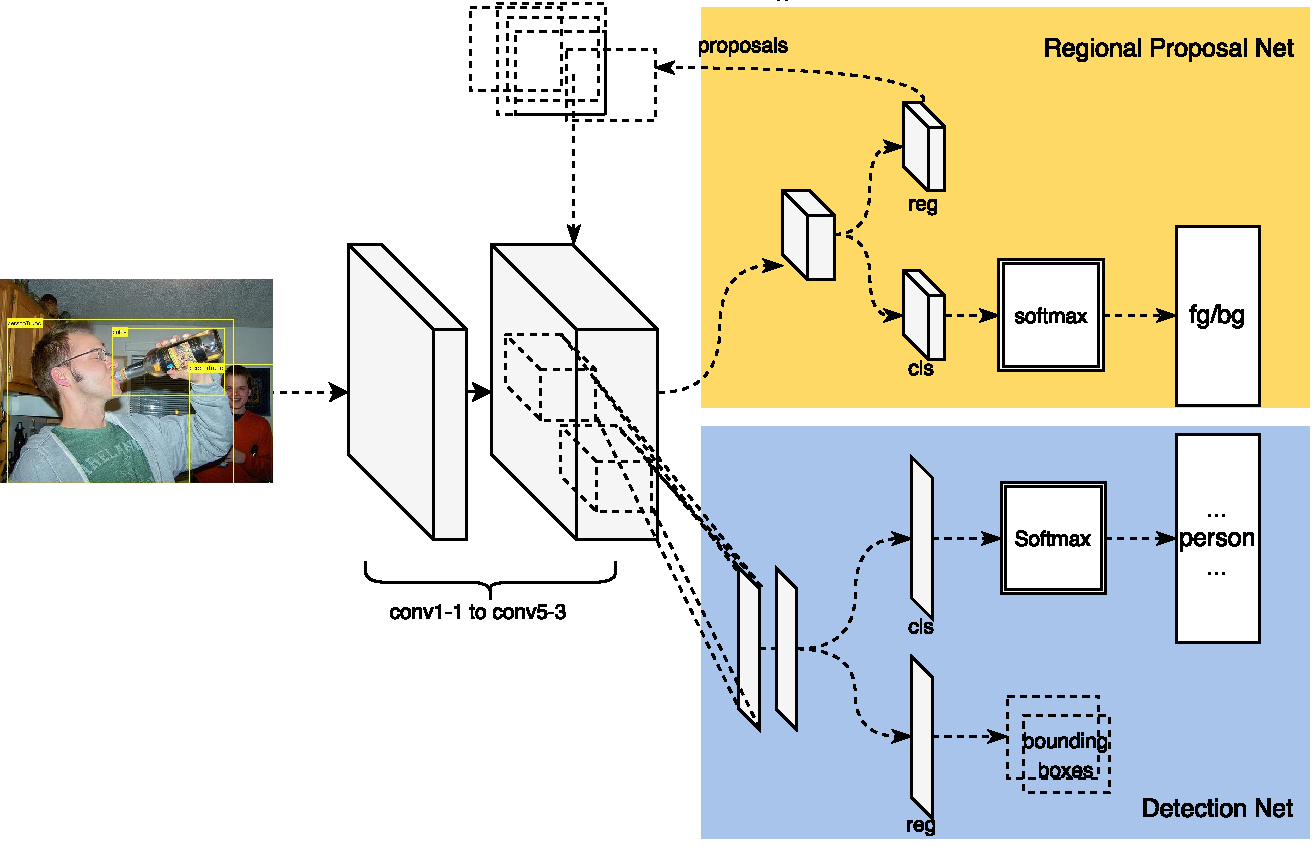
\includegraphics[width=\textwidth]{figures/fasterrcnn.pdf}
	\caption{Architecture of Faster-RCNN.}
	\label{fig:faster-rnn}
\end{figure}
\begin{figure}[h]
	\centering
	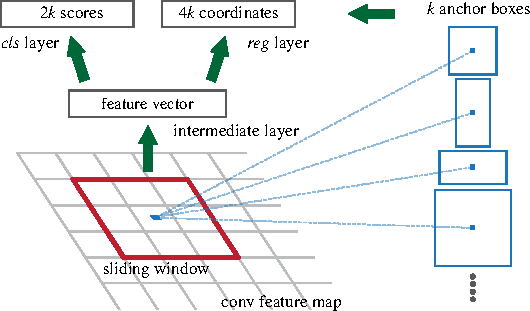
\includegraphics[width=0.7\linewidth]{figures/fasterrcnn-rpn.pdf}
	\caption[Proposal generation in Faster-RCNN]{Proposal generation in Faster-RCNN (slightly modified from source \cite{ren2015faster})}
	\label{fig:rpn}
\end{figure}
\paragraph{RPN} The scheme of proposal generation is depicted in \autoref{fig:rpn} (slightly modified from source \cite{ren2015faster}). 
It takes an input image and generates a set of rectangular regional proposals and 2-tuples corresponding to their binary (foreground/background) prediction.

To generate proposals, a lower-dimensional feature vector $ \mathbf{h}\in \mathbf{R}^d $ is first computed from a small $ n \times n $ neighbourhood of the convolutional feature map (ref the sliding window in \autoref{fig:rpn}) via inner product.
Formally, for an input feature map $ \x $ and weight $ \w $, the $ d $-th entry of the output lower-dimensional vector is computed as
\begin{equation}
\mathbf{h}\left[d\right] = \sum_{\left(w,h\right)\in W,\, k}\x\left[w,h,k\right]\w_{d}\left[w,h,k\right],\label{eq:rpnlowd}
\end{equation}
where $ W $ is the sliding window, $ w $, $ h $ and $ k $ denote the width, height and channel index respectively.

The resultant feature vectors form representations of the corresponding image patch in the input image.
These feature vectors are then fed into two branches of fully connected layers, \textit{cls} and \textit{reg}, for classification (foreground/background) and regression (coordinates of bounding boxes) respectively.

To be specific, at each position of the feature map, $ k $ proposal bounding boxes are generated. 
Those are parameterized relative to $ k $ "anchors", which serve as references for the actual proposals.
Anchors are composed of rectangular regions of various scales and ratios so as to detect objects under scale and size variation.
Faster-RCNN implements 3 scales and 3 ratios, yielding a total of 9 anchors at each position.
In the fully connected layers, $ k $ inner product are carried out independently so that the predictions for each anchor can be computed simultaneously, i.e.
\begin{align}
\mathbf{y}_{cls}[i,k] & = \mathbf{h}^T\w^{cls}_{ik}, \intertext{where $ i\in \lbrace 0,1 \rbrace $ denotes bg and fg labels and}
\mathbf{y}_{reg}[i,k] & = \mathbf{h}^T\w^{reg}_{ik},\label{eq:rpnreg}
\end{align}
where $ i\in \lbrace 0,1,2,3 \rbrace $ denotes the four parameters defining the location of bounding boxes.

On implementation level, since the weights in \autoref{eq:rpnlowd}-\autoref{eq:rpnreg} are shared spatially across all anchor positions, these two steps of inner product can be efficiently realized using two consecutive convolutional layers with kernel size $ n $ and $ 1 $ respectively.

The use of anchor is a novel solution to address multi-scale problem. By creating an individual reference for each scale-ratio combination, it makes it possible to train multi-scale filters simultaneously on a single feature, which serves as the key ingredient for RPN's computation efficiency.

RPN adopts multi-task training same as in DN, i.e. the loss function is a weighted sum of the classification loss $ L_{cls} $ and regression loss $ L_{reg} $. With $ y_{i} $, $ \hat{y}_{i} $, $ \mathbf{t}_{i} $ and $ \hat{\mathbf{t}}_{i} $ denoting the predicted class, groundtruth class, predicted object location (defined as \autoref{eq:bbtuple}) and the groundtruth object location of an anchor $ i $, the loss of the network can be written as
\begin{equation}
L = \dfrac{1}{N_{cls}}\sum_{i}L_{cls}\left(y_{i},\hat{y}_{i}\right) + \lambda \dfrac{1}{N_{reg}}\sum_{i}\hat{y}_{i}L_{reg}\left(\mathbf{t}_{i}, \hat{\mathbf{t}}_{i}\right).
\end{equation}
The classification loss $ L_{cls} $ is the binary softmax loss (see \autoref{eq:softmaxloss}). 
The regression loss $ L_{reg} $ is the smoothed L1 loss introduced in \cite{girshick2015fast}. It is defined as
\begin{align}\label{eq:smoothl1}
L_{reg}\left(\mathbf{t}, \hat{\mathbf{t}}\right) & = \sum_{d=0}^{4}f\left(\mathbf{t}\left[d\right] - \hat{\mathbf{t}}\left[d\right]\right),
\intertext{where $ f $ is the SmoothL1Loss defined as}
f\left(x\right) & = 
\begin{cases}
0.5x^2 & \text{if $ \lvert x \rvert <1 $}\\
\lvert x \rvert - 0.5 & \text{otherwise}
\end{cases}.
\end{align}
While $ L_{cls} $ is comprised of both negative and positive samples, $ L_{reg} $ is contributed only by the positive ones. 
These two terms are normalized with $ N_{cls} $ and $ N_{reg} $ and weighted with hyperparameter $ \lambda $ to ensure balance between the two losses. 
In the current implementation $ \lambda = 10 $, $ N_{cls} $ and $ N_{reg} $ are respectively implemented as the minibatch size (total number of positive and negative samples per image) and the number of anchor positions.

For better training efficiency, samples are constructed with care. 
First of all, to avoid fuzzy samples, labels are assigned using the following rule:
\begin{equation}
\hat{y}_{i} = \begin{cases}
1 & \parbox{0.4\textwidth}{if IoU$ >0.7 $ \\ or \\ $ i $ has the highest IoU with a gt bb}\\
0 & \text{if IoU} <0.3
\end{cases},
\end{equation}
Moreover, since negative samples are dominating, in order to avoid bias towards the negative ones, the samples are assembled with a pos:neg ratio up to 1:1.
\paragraph{DN}
The structure of Detection Network (shown in \autoref{fig:fast-rnn} \cite{girshick2015fast}) remains the same as in Fast-RCNN.

After the last convolutional layer, regional proposals generated from RPN will be used as ROIs in the RoiPooling layer. 
As explained in \autoref{sec:modelarch}, this layer creates a feature map with fixed spatial dimension (e.g. $ 7 \times 7 $) from a rectangular region of arbitrary spatial size. For each proposal, an feature map is generated and are passed to the successive layers as an individual sample.
Two fully connected layers attached on top of the RoiPooling layer compute a large feature vector, which is fed to classification and regression branches in the same fashion as in RPN.

In the loss function, the binary softmax loss is replace by a $ K+1 $ softmax loss, for $ K $ object classes and a catch-all background class. Meanwhile, slight different implementation is taken for the normalizers and weight $ \lambda $: while in DN $ \lambda =1 $, the normalizer is unified between two terms and is implemented as the minibatch size.
\begin{equation}
L = \dfrac{1}{N}\sum_{i}L_{cls}\left(y_{i},\hat{y}_{i}\right) + \lambda \dfrac{1}{N}\sum_{i}\hat{y}_{i}L_{reg}\left(\mathbf{t}_{i}, \hat{\mathbf{t}}_{i}\right).
\end{equation}
\begin{figure}
\centering
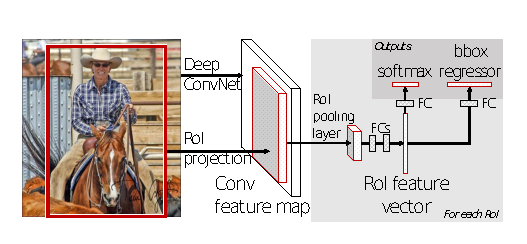
\includegraphics[width=0.7\linewidth]{figures/fast-rnn.eps}
\caption[Detection Network of Faster-RCNN]{Architecture of the Detection Network in Faster-RCNN is completely inherited from Fast-RCNN. The ROIs are generated from Regional Proposal Network. (source \cite{girshick2015fast})}
\label{fig:fast-rnn}
\end{figure}
\paragraph{Training}
The authors of Faster-RCNN has published their trained model for PASCAL VOC detection challenge \cite{pascal-voc-2012}. which contains 20 object classes, including:
person, bird, cat, cow, dog, horse, sheep, aeroplane, bicycle, boat, bus, car, motorbike, train, bottle, chair, dining table, potted plant, sofa, tv/monitor.

Clearly, these 20 classes are far from adequate to serve our purpose, not to mention many of them are inapt for our target action classes (e.g. sheep, potted plant).

Hence we train our own model with expanded object categories.
These are handpicked from ILSVRC2014 \cite{ILSVRC15} (200 categories) and PASCAL VOC \cite{pascal-voc-2012} (20 categories) detection challenge, with exclusion in food, most animals (except horse) and small objects.
This yields 118 categories in total and the complete training data is comprised of 196,780 images.

Since detection network assumes fixed proposals during training, Faster-RCNN adopted a staged training method to achieve layer sharing. This method can be summarized into four steps:
\begin{enumerate}
\item Train a RPN (\texttt{RPN0}) initialized from pre-trained ImageNet VGG16 model \cite{simonyan2014very}.
\item Use \texttt{RPN0} to generate proposals for the same training data;
\item Train a DN (\texttt{DN0}) initialized (again) from ImageNet VGG16 using the proposals generated from the previous step.
\item Train a RPN (\texttt{RPN1}) by fine-tuning the fully connected layers of \texttt{DN0}.
\item Use \texttt{RPN1} to generate proposals from the training data again.
\item Train a DN (\texttt{DN1}) by fine-tuning the fully connected layers of \texttt{DN0} using the newly generated proposals.
\item \texttt{RPN1} and \texttt{DN1} yield the final Faster-RCNN model.
\end{enumerate}

In this thesis, we adopted this staged training method. However, it is worth mentioning, by the time of writing, an update has been published that allows joint training of RPN and DN. 
In this method the proposals generated from RPN branch are fed immediately as pre-computed input into the RoiPooling layer of DN branch \textit{in each iteration step}.
While the proposals in fact are input dependent, this approach does not compute their gradient in back-propagation (RoiPooling function is not w.r.t proposal differentiable), hence called \textit{Approximate joint training}.
Despite of that, this method yields similar results as the staged training and at the same time reduces the training time by $ 25\% \sim 50 \%$.
\subsection{Human Track Extraction}\label{sec:humantrack}
Compared to ImageNet data, frame images in video data have lower resolution and large motion blur. The objects of interest are subject to greater appearance variation as well as temporary occlusion.
Consequently, person detection is inevitably less reliable in video frames. 

Meanwhile, in realistic video datasets videos often contain irrelevant person detections. If used crude, they will add significant amount noise to the training data and consequently increase training difficulty or even affect convergence. 

Thus before deploying the detection results as our model input, we need to pre-process the raw detections so as to
\begin{enumerate}
\item filter out incorrect and irrelevant detections;
\item recover detection failures in individual frames;
\item refine location of bounding boxes.
\end{enumerate}

For these proposes, we propose a simple yet powerful algorithm using the idea of dynamic programming.

We start by characterizing "action relevant" person detections. Contrary to spurious detections, actual action performer displays high overall detectability (except sporadic detection failure) as well as high spatial and appearance consistency in sequential frames. 
In other words, the bounding boxes locating an action performer should form a smooth and continuous "tube" across frames.
\begin{figure}
\centering
\begin{subfigure}{0.25\textwidth}
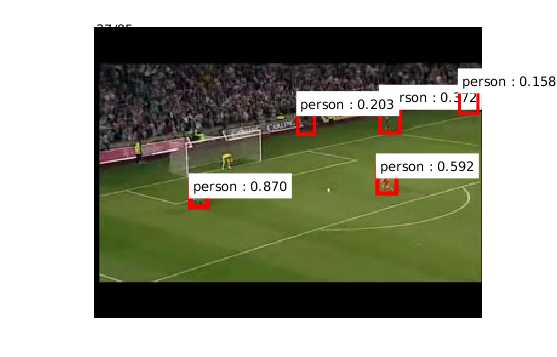
\includegraphics[width=\textwidth, trim={2cm 1.5cm 0cm 1cm}, clip]{figures/soccerpenalty_multi.png}
\end{subfigure}%
\begin{subfigure}{0.25\textwidth}
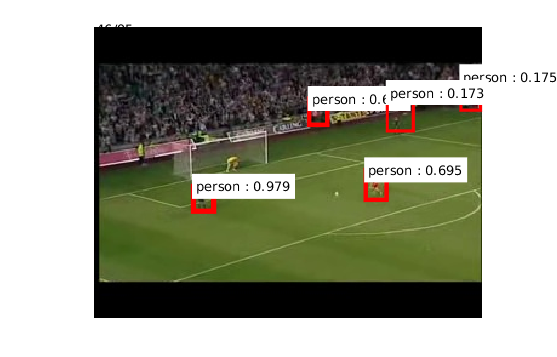
\includegraphics[width=\textwidth, trim={2cm 1.5cm 0cm 1cm}, clip]{figures/soccerpenalty_multi1.png}
\end{subfigure}%
\begin{subfigure}{0.25\textwidth}
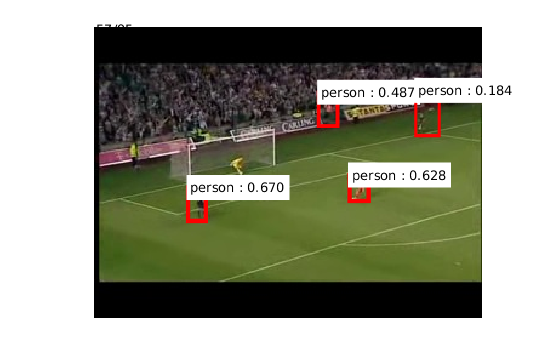
\includegraphics[width=\textwidth, trim={2cm 1.5cm 0cm 1cm}, clip]{figures/soccerpenalty_multi2.png}
\end{subfigure}%
\begin{subfigure}{0.25\textwidth}
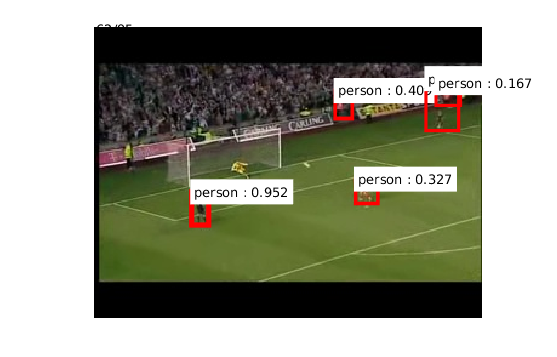
\includegraphics[width=\textwidth, trim={2cm 1.5cm 0cm 1cm}, clip]{figures/soccerpenalty_multi3.png}
\end{subfigure}
\caption[Example of multiple person detections]{An example where incorrect (advertisement) or irrelevant (jury) detections are consistently given by the detector with high confidence. In this case, we use optical flow to pick out the action performer.}\label{fig:multi}
\end{figure}
However, this criterion alone does not suffice. As is shown in \autoref{fig:multi}, wrong detections are often generated consistently with high certainty. 
Nonetheless, while those mostly remain still with the elapse of time, true action protagonist distinguish himself with high motion saliency. 

Inspired by these observations, our task becomes finding a path via raw detections along time axis with the highest detection confidence, temporal consistency and motion saliency. 
These properties can be well expressed quantitatively.
The detectability can be written using the classification probability given by the object detector; 
temporal consistency in location is reflected in form of Intersection over Union (IoU) and the appearance consistency in form of template matching metrics such as Normalized Cross Correlation (NCC); 
motion saliency can be described in terms of optical flow.
Consider each raw detection as a node and the quantitative metrics as costs (or scores) for connections, this problem can be stated as a shortest path problem and solved efficiently with dynamic programming.

Formally, we define the following problem:
\begin{itemize}
\item Given a video of $ T $ frames and the person bounding boxes of this video, we divide the video into $ N = \lfloor\frac{T}{T_{0}}\rfloor$ intervals the length of $ T_{0} $. 
The bounding boxes within the $ n$-th interval construct the state space 
\[ b_{n}^{i}\in\mathcal{B}_{n} \text{ with } n\in\lbrace1,2,\dots, N\rbrace, \] 
$ \mathcal{B}_{n} = \emptyset $ when no person is detected in interval $ n $.
\item the control input $ u_{n} $ at step $ n $ is the choice of bounding box in step $ n+1 $,  while the input space $ \mathcal{U_{n}} $ includes all raw detections and does not depend on the current state, i.e.
\begin{align*}
b_{n+1} & = f_{k}\left(u_{k}\right) \\
u_{k} & \in \lbrace 1, 2, \dots, \lvert \mathcal{B} \rvert\rbrace.
\end{align*}
\item the score $ s_{ij} $ for connecting two bounding boxes $ b^{i}_{n} $ and $ b^{j}_{n+1} $ consecutive intervals $ n $ and $ n+1 $ is defined as
\begin{equation}
s_{ij}\left(b^{i}_{n}, b^{j}_{n+1}\right) = s_{prob}\left(b^{j}_{n+1}\right) + s_{motion}\left(b^{j}_{n+1}\right)+ s_{IoU}\left(b^{i}_{n}, b^{j}_{n+1}\right) + s_{size}\left(b^{j}_{n+1}\right).
\end{equation}
\begin{itemize}
\item $ s_{prob} $ is the probability with which bounding box $ b_{n+1}^{j} $ is classified as person, describing detection certainty
\begin{equation}
s_{prob}\left(b^{j}_{n+1}\right) = \Pr\left(c^{j}=\text{person}|b^{j}_{n+1}\right).
\end{equation} 
\item $ s_{IoU} $ is a function of IoU of the two concerned bounding boxes,  aimed to reflect the temporal consistency
\begin{equation}
s_{IoU}\left(b^{i}_{n}, b^{j}_{n+1}\right) = 
\begin{cases}
IoU\left(b^{i}_{n}, b^{j}_{n+1}\right) & \text{if } IoU\left(b^{i}_{n}, b^{j}_{n+1}\right)>0\\
-c \text{ with } c>0 & \text{otherwise}.
\end{cases}.
\end{equation}
\item $ s_{motion} $ is the average of the normalized magnitude of optical flow in area $ b_{n+1}^{j} $, describing motion saliency 
\begin{equation}
s_{motion}\left(b^{j}_{n+1}\right) = \dfrac{1}{\lvert b_{n+1}^{j}\rvert}\sum_{\left(x,y\right)\in b_{n+1}^{j}}\lVert o\left(x,y\right) \rVert
\end{equation}
\item $ s_{size}\left( b^{j}_{n+1}\right) $ puts additional penalty on small bounding boxes. This proves to be useful in complex scenes since the action performer is usually the most prominent among all detected person.
\begin{equation}
s_{size}\left(b^{j}_{n+1}\right) = f\left( \dfrac{\vert b^{k}_{n+1}\rvert}{\max_{k} \vert b^{k}_{n+1}\rvert}\right),
\end{equation}
where $ f $, shown in \autoref{fig:non-linearf}, is a sigmoid-like non-linear mapping to suppress small regions, while preserving the large ones.
A sigmoid function has the form
\begin{equation}
f\left(x\right)=\dfrac{L}{1+\exp\left(-k\left(x-x_{0}\right)\right)}.
\end{equation}
In our implementation, we set the parameters to
\begin{equation}
x_{0}=0.5 \quad k = 12 \quad L=0.5.
\end{equation}
While $ x $ and $ k$ are set so to keep the x-span of the ``S'' shape within $ \left[0,1\right] $, so as to comply with the input range, $ L $ is determined from empirical test results.
\end{itemize}
\item Finally we consider the following optimization problem:
\begin{equation}
\max_{\pi}\left(\sum_{n=1}^{N}s_{ij}\left(b^{i}_{n}, b^{j}_{n+1}\right)\right),
\end{equation}
where $ \pi $ denotes a sequence of bounding boxes selected from each interval.
\end{itemize}
\begin{figure}[h]
	\centering
	\begin{tikzpicture}
	\begin{axis}[
	axis lines=middle,
	ymin=0,ymax=1,
	xmin=0,xmax=1,
	xlabel={relative size},
	]
	\addplot[mark=none, samples=200, smooth] plot{1/(1+exp(-12*(x-0.5)))};
	\end{axis}
	\end{tikzpicture}
	\caption[Size penalty for action performer extraction]{Although the relative size of a detected person gives hint to his relevancy, our experiment suggests this relation is not linear. Hence we apply a sigmoid-like threshold function to suppress only very small bounding boxes.}
	\label{fig:non-linearf}
\end{figure}

This problem can be solved efficiently using dynamic programming by applying \autoref{eq:recursion} from \autoref{sec:dp} ($ \max $ instead of $ \min $). 

The optimal policy $ \pi^{*} $ is a sequence of $ N $ bounding boxes. The frames, from which the bounding boxes are chosen, form a set of \textit{key frames}. From these key frames, we apply a linear ex-interpolation on the four coordinates of the bounding boxes to obtain a smooth track of the person of interest in the whole video span. 

There is one noteworthy design choice in our method. 
As an alternative to the natural choice to treat each frame as a time step, we group multiple consecutive frames to form a single step, thus implicitly increase the state space at each step $ \mathcal{B}_{n} $.
As a result, we are able to "look ahead" when no feasible solution exist at current frame.
This introduced flexibility is the key to recover detection failures and correct faulty detections.

An example of resulted person track is shown in \autoref{fig:persontrack}. As we can see, our method successfully recognizes the action performer among multiple people detections and fix detection failures even under large temporal gap.

\begin{figure}[h]
  \centering
\begin{subfigure}{0.12\textwidth}
	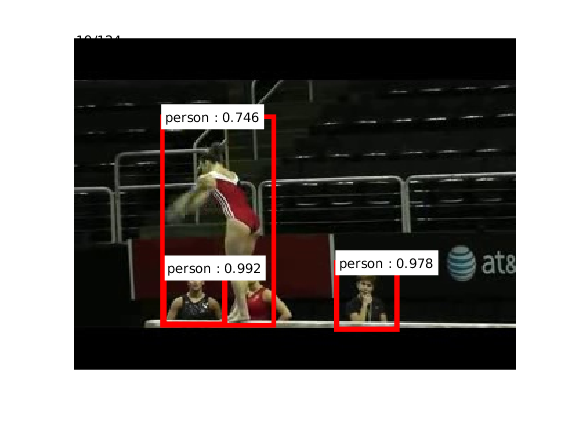
\includegraphics[width=\textwidth,trim={2cm 1cm 2cm 1cm},clip]{figures/person_tube_raw_0.png}
\end{subfigure}%
\begin{subfigure}{0.12\textwidth}
	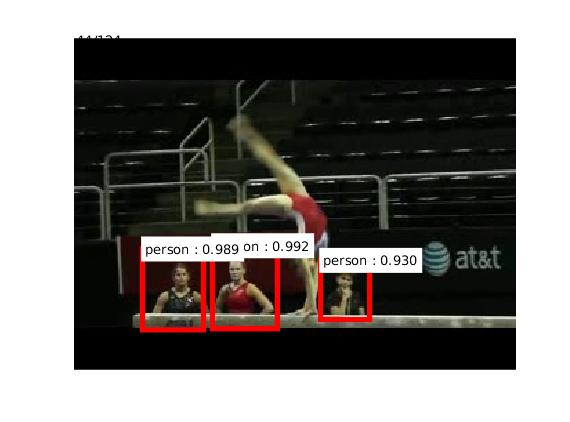
\includegraphics[width=\textwidth,trim={2cm 1cm 2cm 1cm},clip]{figures/person_tube_raw_3.png}
\end{subfigure}%
\begin{subfigure}{0.12\textwidth}
	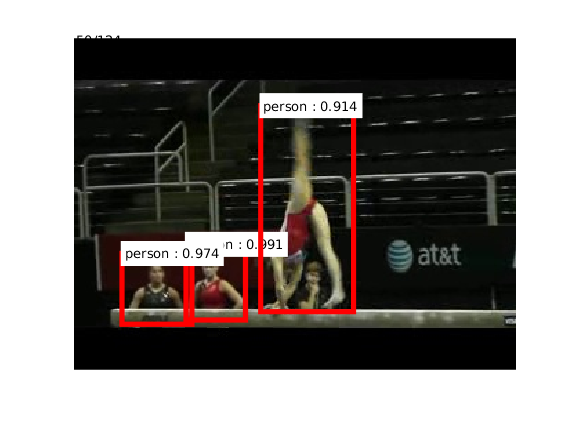
\includegraphics[width=\textwidth,trim={2cm 1cm 2cm 1cm},clip]{figures/person_tube_raw_4.png}
\end{subfigure}%
\begin{subfigure}{0.12\textwidth}
	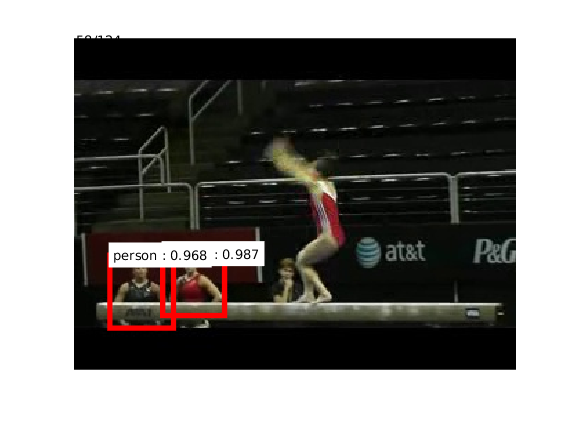
\includegraphics[width=\textwidth,trim={2cm 1cm 2cm 1cm},clip]{figures/person_tube_raw_5.png}
\end{subfigure}%
\begin{subfigure}{0.12\textwidth}
	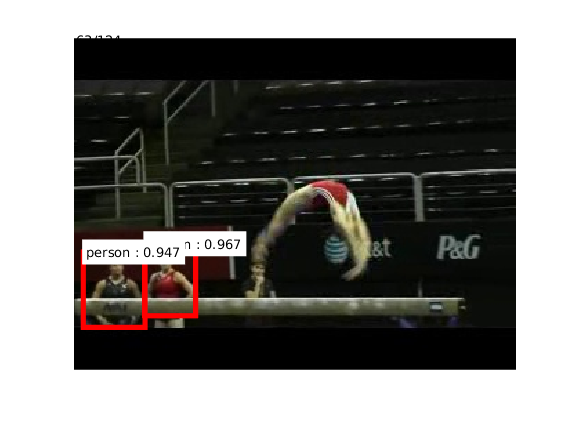
\includegraphics[width=\textwidth,trim={2cm 1cm 2cm 1cm},clip]{figures/person_tube_raw_6.png}
\end{subfigure}%
\begin{subfigure}{0.12\textwidth}
	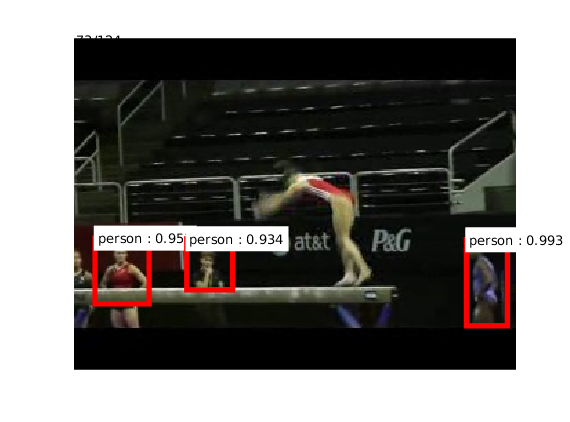
\includegraphics[width=\textwidth,trim={2cm 1cm 2cm 1cm},clip]{figures/person_tube_raw_8.png}
\end{subfigure}%
\begin{subfigure}{0.12\textwidth}
	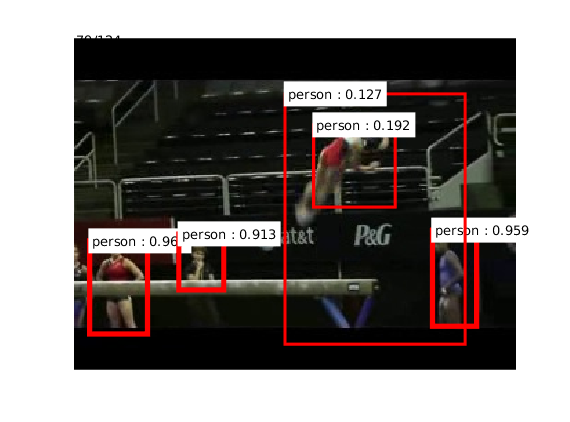
\includegraphics[width=\textwidth,trim={2cm 1cm 2cm 1cm},clip]{figures/person_tube_raw_9.png}
\end{subfigure}%
\begin{subfigure}{0.12\textwidth}
	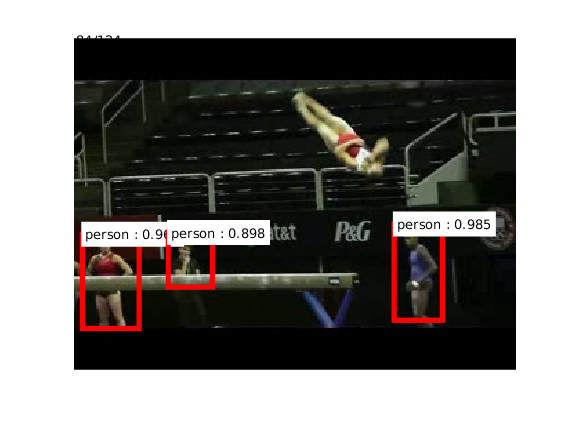
\includegraphics[width=\textwidth,trim={2cm 1cm 2cm 1cm},clip]{figures/person_tube_raw_10.png}
\end{subfigure}
\begin{subfigure}{0.12\textwidth}
	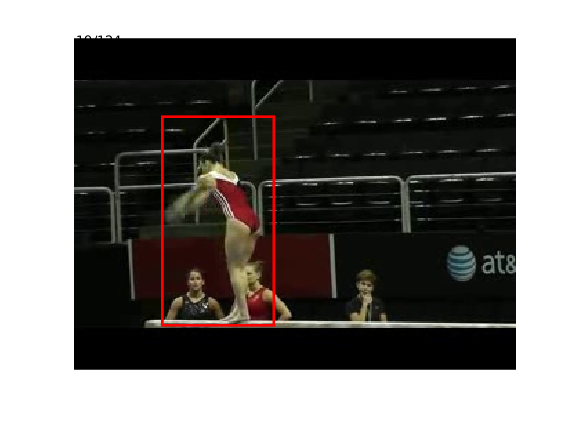
\includegraphics[width=\textwidth,trim={2cm 1cm 2cm 1cm},clip]{figures/person_tube_0.png}
\end{subfigure}%
\begin{subfigure}{0.12\textwidth}
	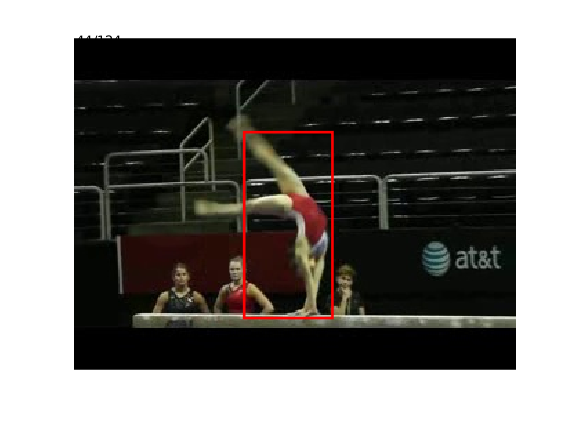
\includegraphics[width=\textwidth,trim={2cm 1cm 2cm 1cm},clip]{figures/person_tube_3.png}
\end{subfigure}%
\begin{subfigure}{0.12\textwidth}
	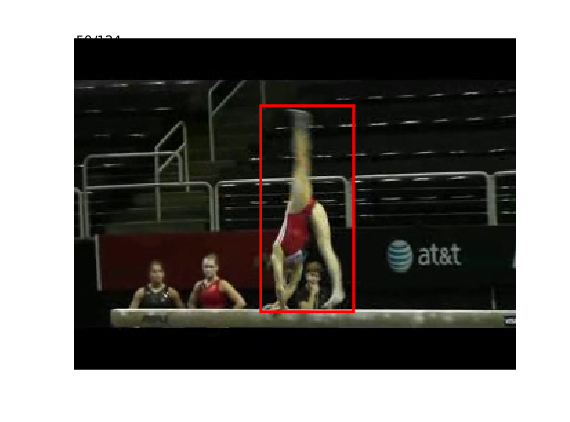
\includegraphics[width=\textwidth,trim={2cm 1cm 2cm 1cm},clip]{figures/person_tube_4.png}
\end{subfigure}%
\begin{subfigure}{0.12\textwidth}
	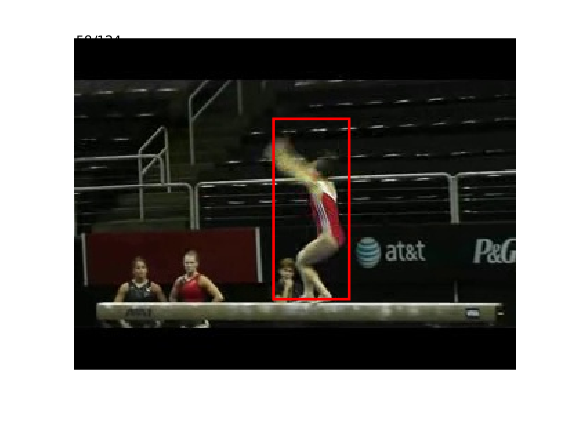
\includegraphics[width=\textwidth,trim={2cm 1cm 2cm 1cm},clip]{figures/person_tube_5.png}
\end{subfigure}%
\begin{subfigure}{0.12\textwidth}
	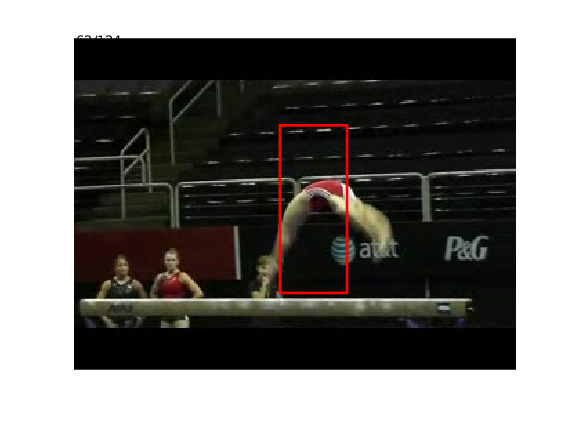
\includegraphics[width=\textwidth,trim={2cm 1cm 2cm 1cm},clip]{figures/person_tube_6.png}
\end{subfigure}%
\begin{subfigure}{0.12\textwidth}
	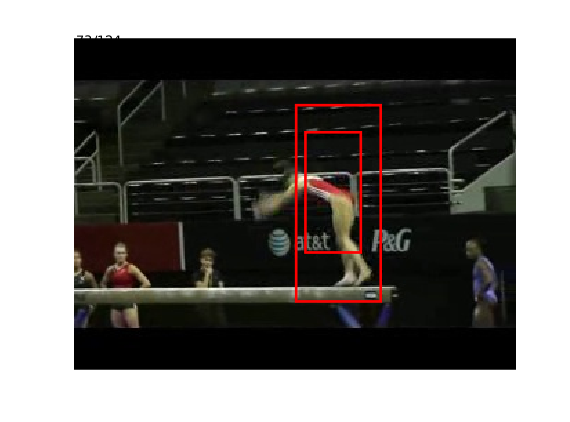
\includegraphics[width=\textwidth,trim={2cm 1cm 2cm 1cm},clip]{figures/person_tube_8.png}
\end{subfigure}%
\begin{subfigure}{0.12\textwidth}
	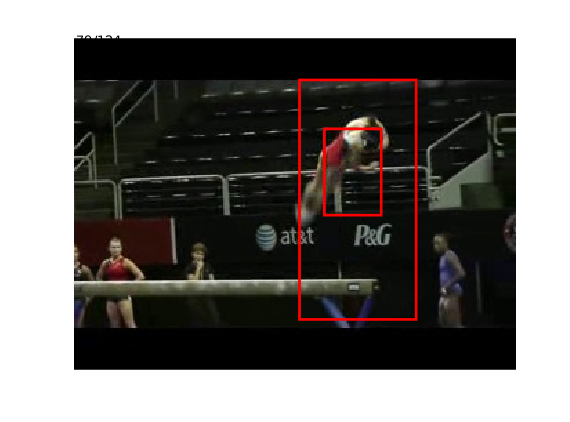
\includegraphics[width=\textwidth,trim={2cm 1cm 2cm 1cm},clip]{figures/person_tube_9.png}
\end{subfigure}%
\begin{subfigure}{0.12\textwidth}
	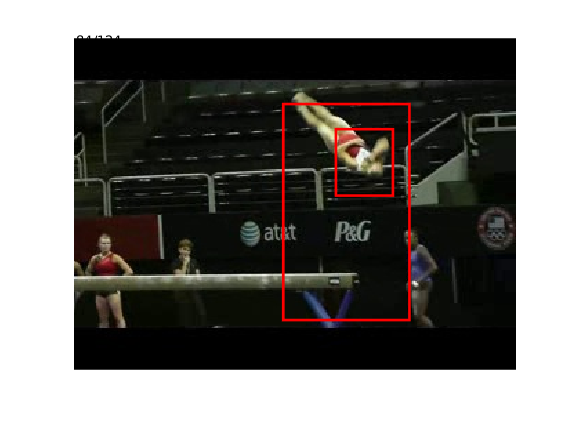
\includegraphics[width=\textwidth,trim={2cm 1cm 2cm 1cm},clip]{figures/person_tube_10.png}
\end{subfigure}
\caption[An sample result of action performer extraction]{An example of the resulted person track using our algorithm. 
Compared to the raw detections (upper row), our method is able to filter out noisy detections and recover missing frames, despite detection failures over a long period and confident detections of irrelevant people.}\label{fig:persontrack}
\end{figure}

Although in most cases we are able to locate the action performer from the optimal track determined by our algorithm, exceptions reside especially in action classes where multiple people are involved or overlapped. 
In this case, we need to find another track that is independent from the previous one. 
We stress independent here, since in the concerned situation the interested person tracks are often intertwined.
As a result, simply returning the second optimal solution from dynamic programming would have resulted in a mixed track, partially containing the already extracted one (see \autoref{fig:interception} for a concrete example).

\begin{figure}[h]
\centering
\begin{tikzpicture}
[>=stealth]
\matrix (m) [
matrix of math nodes, 
nodes={draw, circle, minimum size=1cm},
row 1/.style={nodes={teal}},
row 3/.style={nodes={red}},
row sep={1cm,between origins},
column sep={1cm}
]
{
a_{1} & a_{2} &  & a_{4} \\
 &  & |[draw=red, pattern=north east lines ,pattern color=teal]| ab_{3}& \\
b_{1} & b_{2} &  & b_{4}\\
};
\node [below=of m-3-1](t1) {step $ 1 $};
\node [below=of m-3-2](t2) {step $ 2 $};
\node [right=of t2](t3) {step $ 3 $};
\node [below=of m-3-4](t4) {step $ 4 $};
\draw [->, teal] ([xshift=-1cm]m-1-1.west) -- (m-1-1) --node[above] {4.5} (m-1-2) -- node[above] {3.8} (m-2-3) -- node[above] {1.8} (m-1-4);
\draw [->, red] ([xshift=-1cm]m-3-1.west) -- (m-3-1) -- node[above] {4.3}(m-3-2) -- node[above] {3.5} (m-2-3) -- node[above] {1.5} (m-3-4);
\end{tikzpicture}
\caption[Finding the multiple person tracks]{Illustration of two person tracks that are intercepted at one frame. 
Red and green represent the tracks of person $ a $ and $ b $, and the green one is apparently the optimal track. 
However if we want to extract person $ b $ additionally by simply backtracking from the node with the second highest score (in this case $ b_{1} $) in step $ 1 $, we will end up with the track $ b_{1}-b_{2}-a_{3}-b_{4} $.} \label{fig:interception}
\end{figure}

We solve this problem by eliminating the first person track (and bounding boxes that highly overlap with it) from the available raw detection, while preserving the interception bounding box (the shadowed node in \autoref{fig:interception}). 
From this reduced state space, we repeat dynamic programming algorithm to extract the second person track. An example of the resulting person tracks is shown in \autoref{fig:top2person}.
\begin{figure}
\centering
\begin{subfigure}{0.3\linewidth}
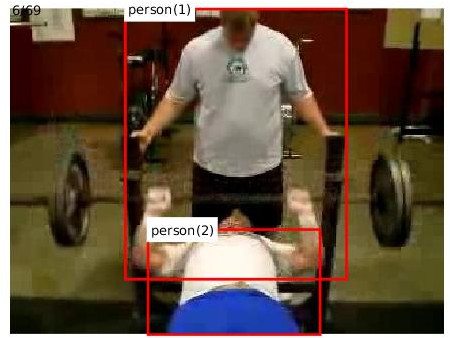
\includegraphics[width=\textwidth]{figures/benchpress.jpg}
\end{subfigure}%
\begin{subfigure}{0.3\linewidth}
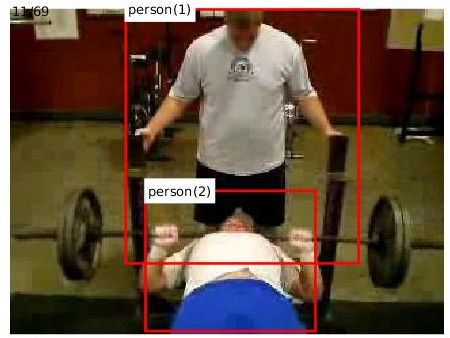
\includegraphics[width=\textwidth]{figures/benchpress2.jpg}
\end{subfigure}%
\begin{subfigure}{0.3\linewidth}
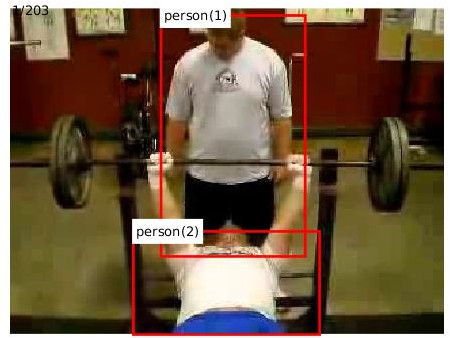
\includegraphics[width=\textwidth]{figures/benchpress3.jpg}
\end{subfigure} 
\caption[Multiple independent person tracks]{An example where multiple individual person tracks, partially overlapping, are extracted.}\label{fig:top2person}
\end{figure}

The complete algorithm is summarized in \autoref{alg:persontrack}. Notice that small adaptation is implemented to handle intervals void of detections ($ \mathcal{B}_{n} = \emptyset $). 
Additionally, score-filtering as well as early termination condition are added for the sake of computation efficiency.

\begin{algorithm}[b]
\small
	\caption{Top-K Person Track Extraction}
	\label{alg:persontrack}
	\begin{algorithmic}[1]
		\State \textbf{Output}: $ metricThreshold $
		\State \textbf{Input:} 
		\NewLine $ T $ RGB video frames, 
		\NewLine $ 2T $ flow images, 
		\NewLine $ T $ sets of bounding boxes from raw person detection $\lbrace \mathcal{B}_{t} \rbrace_{1}^{T}$
		\If{$ p\left(person|b\right) < s_{min}$} \Comment{Filter very uncertain detections}
		\State remove $ b $ from $\lbrace \mathcal{B}_{t} \rbrace_{1}^{T}$
		\EndIf
		\State \textbf{Parameter}: $ T_{0} $, $ s_{min} $, $ K $
		\For{$ 1 $ to $ K $} \Comment{Top-K person tracks}
		\State group $\lbrace \mathcal{B}_{t} \rbrace_{1}^{T}$ into $ \lfloor \frac{T}{T_{0}}\rfloor $ intervals, $ \lbrace \mathcal{B}_{i}\rbrace_{1}^{N} $
		\State remove empty intervals and get $ \lbrace \mathcal{B}'_{i}\rbrace_{1}^{N'}\, s.t. \mathcal{B}'_{i} \not = \emptyset$
		\If {$ N' \leq \frac{N}{2} $}
			\Break
		\EndIf
		\Procedure{Dynamic Programming}{flow, $ \lbrace \mathcal{B}'_{i}\rbrace_{1}^{N'}$}
		\State $ J_{N'}\left(b_{N'}^{i}\right) = s_{prob}\left(b^{i}_{N'}\right) + s_{motion}\left(b^{i}_{N'}\right)+ s_{size}\left(b^{i}_{N'}\right).$
		\Repeat
		\State Apply dynamic programming recursion:
		\NewLine $  J_{n}\left(b_{n}^{i}\right) = \max_{j} \left(s_{ij}\left(b_{n}^{i}, b_{n+1}^{j}\right) +  J_{n+1}\left(b_{n+1}^{j}\right)\right)$
		\NewLine $ \mu_{n}^{*}\left(b_{n}^{i}\right) = \argmax_{j} \left(s_{ij}\left(b_{n}^{i}, b_{n+1}^{j}\right) +  J_{n+1}\left(b_{n+1}^{j}\right)\right) $
		\Until {$ k=1 $}
		\If {$ \max_{i} J_{1}\left(b_{1}^{i}\right) < 0$} \Comment{soft constraint}
		\Break
		\EndIf
		\State forward trace $ \lbrace \mu_{n}^{*}\rbrace_{1}^{N'}$ to get $ \pi^{*} = \lbrace b_{1}^{*}, b_{2}^{*}, \dots b_{N'}^{*}\rbrace$
		\EndProcedure
		\State linear ex-interpolate from $ \pi^{*} $ to get $ \pi^{**} = \lbrace b_{t}^{*}\rbrace_{1}^{T}$
		\LineComment{remove found person track according to \autoref{fig:interception}}
		\For{$t = 1 $ to $ T $}
		\If{$ IoU\left(b_{t}^{i}, b_{t}^{*}\right) > 0.8 $  \textbf{and} $\not\exists j\not = k, \, s.t. \mu(b_{t-1}^{j}) = \mu(b_{t-1}^{k}) =  b_{t}^{i} $}
		\State remove $ b_{t}^{i} $ from $ \mathcal{B}_{t} $
		\EndIf
		\EndFor
		\EndFor
	\end{algorithmic}
\end{algorithm}

\subsection{Object Filtering}\label{sec:objectfilter}
Due to much larger variance and complexity presented in video, meanwhile refrained by the number of target object categories, detection results for objects are inevitably less reliable than for human. 
On the other hand, drawing a clear line between relevant and irrelevant objects is not possible. 
As a matter of fact, as mentioned in \cite{jain201515}, while the existence of certain object categories matter, the absence of them provides useful information as well.
While manually matching object categories with action classes is feasible, such approach is not suited for general scenarios.

\begin{figure}
\centering
\begin{subfigure}{0.3\linewidth}
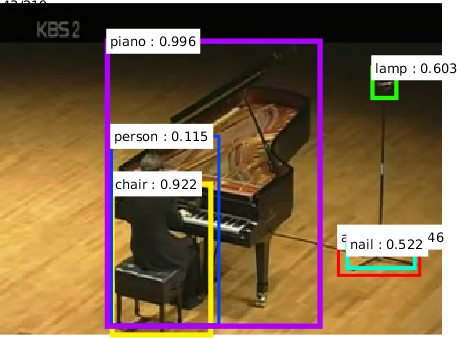
\includegraphics[width=\columnwidth]{figures/obj_detect2.png}
\end{subfigure}
\begin{subfigure}{0.3\linewidth}
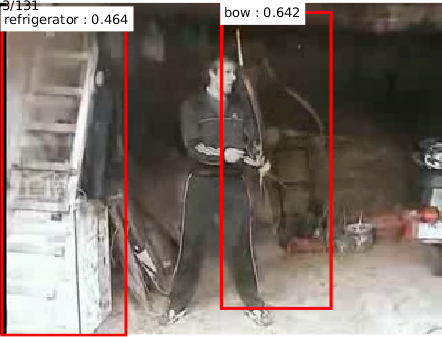
\includegraphics[width=\columnwidth]{figures/obj_detect3.png}
\end{subfigure}
\begin{subfigure}{0.3\linewidth}
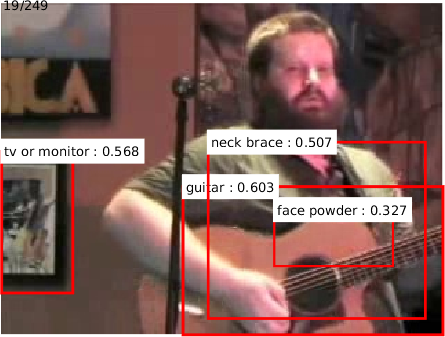
\includegraphics[width=\columnwidth]{figures/obj_detect5.png}
\end{subfigure}
\caption[Object detection examples]{Examples of object detection results}\label{fig:objdetection}
\end{figure}
However as the examples in \autoref{fig:objdetection} shows, the classification probability is usually a good indicator on how substantial the detected object is.
Meanwhile the size of the object and its distance to human gives important hints to the relevance of the object.

From these observations, we first eliminate all objects whose largest prediction probability lower than $ 0.1 $ then we exclude bounding boxes with length smaller than $ 20 $ pixels.
In the frames existence of any actor, we further filter out objects that do not overlap with any detected action performer.
The remaining detected objects comprise ROIs for object channel.

In \autoref{fig:filteredbb}, we show some examples of filtered object detections.
\begin{figure}
\centering
\begin{subfigure}{0.3\linewidth}
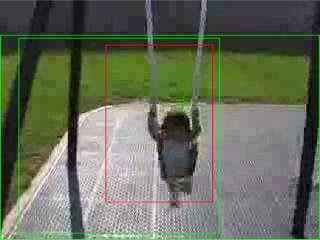
\includegraphics[width=\columnwidth]{figures/netinput.png}
\end{subfigure}
\begin{subfigure}{0.3\linewidth}
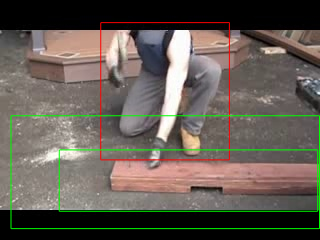
\includegraphics[width=\columnwidth]{figures/netinput_hammer.png}
\end{subfigure}
\begin{subfigure}{0.3\linewidth}
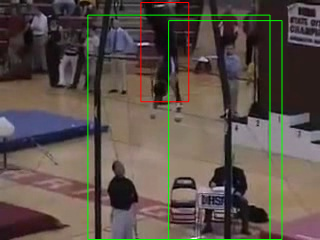
\includegraphics[width=\columnwidth]{figures/netinput_stillring.png}
\end{subfigure}
\caption[Examples of Bounding Box Inputs]{Examples of filtered bounding boxes.}\label{fig:filteredbb}
\end{figure}

\section{Merging Unit}\label{sec:fusion}
Obvious, different semantic cue impact the understanding and interpretation of each individual type of actions with different weights.
Hence, one main focus in this thesis is to find a sophisticated way to integrate them together.

For the purpose, we propose 6 kinds of fusion methods.
Assume we have $ C $ action classes and $ L $ semantic channels, the classification score generated by channel $ l $ is denoted as $ s_{l}\in \mathbb{R}^C $, then we have:
\begin{enumerate}
\item \textbf{sum}: the classification score of class $ c $ is the summation over all available cues.
\begin{equation}
s\left[c\right] = \sum_{l=1}^{L}s_{l}\left[c\right].
\end{equation}
In back-propagation, loss gradient is equally passed to all cues. Implicitly, this assumes that all cues have equal contributions to the final decision.
\item \textbf{max}: instead of summing the classification scores, one can also apply max operation. 
Intuitively, this is equivalent as picking the strongest cue for each action class as the final class representation.
Recall the MaxPooling operation discussed in \ref{sec:cnnlayers}, during back-propagation gradient from upper layer is passed down only to the corresponding cue, from which the maximum value is pooled.
As a result, each cue will be updated according to its actual contribution.
Formally, 
\begin{equation}
s\left[c\right] = \max_{l=1}^{L}s_{l}\left[c\right].
\end{equation}
It should be noted, this fusion is equivalent to the MIL merge we use for object cue (see \autoref{sec:modelarch}). 
In this case, results from different cues are instances in a bag.
\item \textbf{weighted} The drawback of sum fusion is that it treats all cues equally across all action classes. 
In reality, this is not true in most cases, e.g. person in "JumpingRope" has much higher relative importance than person in "HorseRace".
To address the issue, we propose weighted fusion, namely
\begin{equation}
s\left[c\right] = \sum_{l=1}^{L}w_{l}[c]s_{l}\left[c\right],
\end{equation}
There are a total $ L\times C$ weights and $ w_{l}\left[c\right] $ is the weight of the $ l $-th cue for class $ c $.
\item \textbf{cross-weighted}
Moreover, we experiment with the cross-class joint weighting same as in \cite{xiong2015recognize}.
In other words, the final classification score is determined by the classification results of all cues and all classes.
This setting incorporates extra information from class confusions and exclusions. 
For example, if a sample frame has strong response to "Kayaking" from scene channel, then a smaller weight should be assigned to "HorseRace" in person channel.
Formally, the final score can be written as
\begin{equation}
s\left[c\right] = \sum_{l=1}^{L}\sum_{c'=1}^{C}w_{l}\left[c,c'\right] s_{l}\left[c'\right].
\end{equation}
There are in total $ L \times C \times C $ weights. 
\item \textbf{multi-loss} 
Besides the above fusion methods, we also explored with multi-tasking training scheme implemented in Fast-RCNN. 
Classification using each semantic cue is regarded as a separate task.
In forward pass, each cue generates a loss independently as illustrated in \autoref{fig:multiloss}, whose gradients are passed down through the corresponding fc branch and combined before the shared convolutional layer.
For testing, we compute the final prediction via either summation or maximization.
\item \textbf{multi-loss+}
At last, as depicted in \autoref{fig:multiloss+} we combine the multi-tasking with fusion unit, where the choice fusion unit is determined by the result of above comparisons.
While this architecture still uses the merged result as final classification decision, separate losses are used as constraints to guarantee single-cue performance.
In order to emphasis the importance of merged result, we assign a higher weight to the merged loss. 
As a result, the parameters will be updated more in favour of the merged result.
\end{enumerate}

\begin{figure}[h]
\begin{subfigure}[b]{0.5\linewidth}
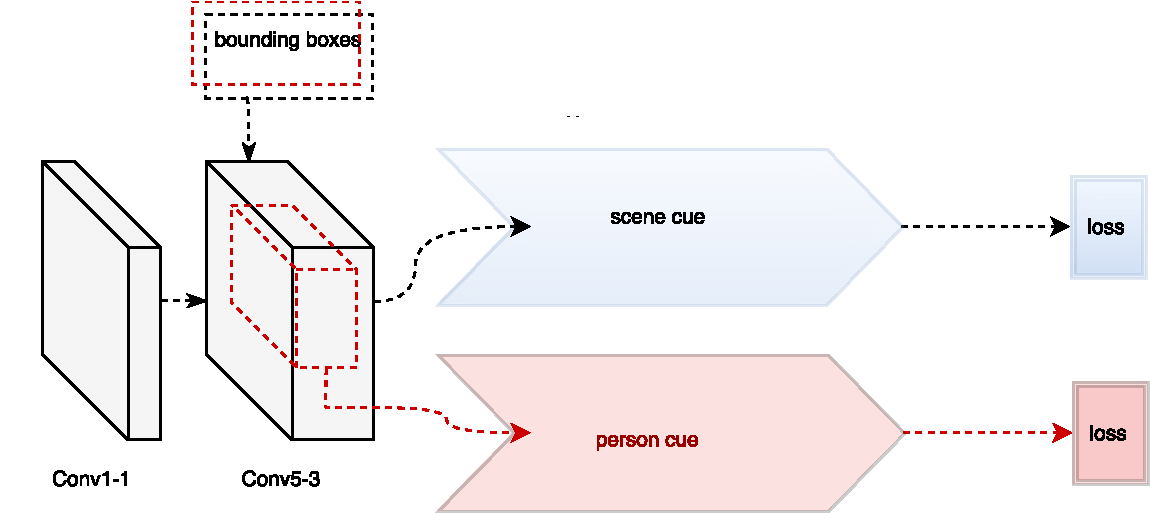
\includegraphics[width=\columnwidth]{figures/multiloss}
\subcaption{Multi-loss Fusion}\label{fig:multiloss}
\end{subfigure}
\begin{subfigure}[b]{0.5\linewidth}
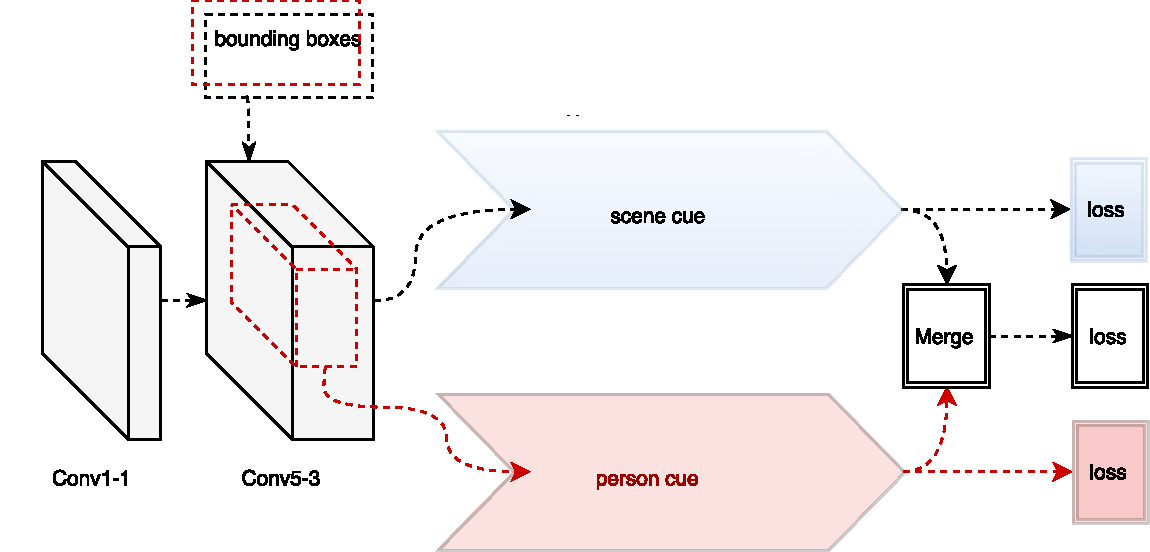
\includegraphics[width=\columnwidth]{figures/multiloss+}
\subcaption{Multi-loss+ Fusion}\label{fig:multiloss+}
\end{subfigure}
\caption[Multiloss Fusion Variants]{Architectures for multi-loss fusion proposals.}
\end{figure}